%
% $RCSfile: system.tex,v $
%
% Copyright (C) 2002-2008. Christian Heller.
%
% Permission is granted to copy, distribute and/or modify this document
% under the terms of the GNU Free Documentation License, Version 1.1 or
% any later version published by the Free Software Foundation; with no
% Invariant Sections, with no Front-Cover Texts and with no Back-Cover
% Texts. A copy of the license is included in the section entitled
% "GNU Free Documentation License".
%
% http://www.cybop.net
% - Cybernetics Oriented Programming -
%
% http://www.resmedicinae.org
% - Information in Medicine -
%
% Version: $Revision: 1.1 $ $Date: 2008-08-19 20:41:09 $ $Author: christian $
% Authors: Christian Heller <christian.heller@tuxtax.de>
%

\subsection{System}
\label{system_heading}
\index{System}
\index{Knowledge}
\index{Input of a System}
\index{Output of a System}
\index{Behaviour}

Earth is a system, a biotope and its biological creatures, including human
beings, are systems, our society, institutions, families and their individuals
are systems, machines and computers are systems -- and software applications
are systems. Actually, almost everything in existence can be treated and
simulated as system.

A rather general definition \cite{wikipedia} describes a system as: \textit{an
assemblage of inter-related elements comprising a unified whole.} Systems are
in a steady exchange with their environment. Information systems, for example,
exchange data. Depending on their structure, relations and contents, these may
be called \emph{Knowledge}. From the view of a system, the data are called
\emph{Input} and \emph{Output}. The output of one system can become the input
for another.

A certain logic with special rules can be abstracted in form of a \emph{System}.
The system's logic causes its characteristic \emph{Behaviour}, that is the way
its \emph{Input} gets manipulated to produce a specific \emph{Output}.

%
% $RCSfile: deterministic_and_stochastic_behaviour.tex,v $
%
% Copyright (C) 2002-2008. Christian Heller.
%
% Permission is granted to copy, distribute and/or modify this document
% under the terms of the GNU Free Documentation License, Version 1.1 or
% any later version published by the Free Software Foundation; with no
% Invariant Sections, with no Front-Cover Texts and with no Back-Cover
% Texts. A copy of the license is included in the section entitled
% "GNU Free Documentation License".
%
% http://www.cybop.net
% - Cybernetics Oriented Programming -
%
% http://www.resmedicinae.org
% - Information in Medicine -
%
% Version: $Revision: 1.1 $ $Date: 2008-08-19 20:41:06 $ $Author: christian $
% Authors: Christian Heller <christian.heller@tuxtax.de>
%

\subsubsection{Deterministic- and Stochastic Behaviour}
\label{deterministic_and_stochastic_behaviour_heading}
\index{Deterministic Behaviour}
\index{Stochastic Behaviour}
\index{Probabilistic Behaviour}
\index{Fuzzy Logic}
\index{Artificial Neural Network}
\index{ANN}

Systems can be distinguished by their behaviour, which can be \emph{deterministic}
or \emph{stochastic} (probabilistic). While the elements of the first work in a
predictable way, probabilistic systems are not fully transparent and their
results are only \emph{likely}, but never \emph{certain}. Living systems are
entirely probabilistic, because firstly, not all of their elements are known
and secondly, they always consist of sub systems on different functional
levels. \cite{sengbusch}

Two areas dealing with the simulation of stochastic behaviour are \emph{Fuzzy Logic}
%(section \ref{fuzzy_logic_heading})
and \emph{Artificial Neural Networks} (ANN).
%(section \ref{artificial_neural_network_heading}).
Most software systems
though, need \emph{reliable} (deterministic) behaviour delivering
\emph{predictable} results. Deterministic systems are therefore in the focus of
the research done in this work.

%
% $RCSfile: black_box.tex,v $
%
% Copyright (C) 2002-2008. Christian Heller.
%
% Permission is granted to copy, distribute and/or modify this document
% under the terms of the GNU Free Documentation License, Version 1.1 or
% any later version published by the Free Software Foundation; with no
% Invariant Sections, with no Front-Cover Texts and with no Back-Cover
% Texts. A copy of the license is included in the section entitled
% "GNU Free Documentation License".
%
% http://www.cybop.net
% - Cybernetics Oriented Programming -
%
% http://www.resmedicinae.org
% - Information in Medicine -
%
% Version: $Revision: 1.1 $ $Date: 2008-08-19 20:41:05 $ $Author: christian $
% Authors: Christian Heller <christian.heller@tuxtax.de>
%

\subsubsection{Black Box}
\label{black_box_heading}
\index{Black Box}
\index{Operation}
\index{Functional Elements}
\index{Complexity Hiding}
\index{Block Diagram}
\index{Unified Modeling Language}
\index{UML}

An \emph{Operation} can be well treated as system: it contains rules of logic
after which its input gets transformed into its output. But not all systems are
as easy as a simple operation; many are \emph{composed} of yet smaller systems.
Biological systems, for example, are extremely difficult to describe in their
entirety, with a simple mathematical formula.

A system may be seen as a number of interacting \emph{Functional Elements}. It
is these elements and their interactions which determine the specific
properties and behaviour of a system. However, for modelling the behaviour of a
transmission system, its inner structure is not important. Systems theory
focusses on the time-dependent progression of input- and output signals as well
as their relation.

A common technique in systems engineering is to reduce complexity by
\emph{hiding} functionality which is unimportant in the given context, inside a
system. One then talks of a system as \emph{Black Box} since only its input,
output and their relation, but not its inside, are considered (figure
\ref{blackbox_figure}). The black box provides an encapsulation towards the
infinite microcosm, and it knows nothing about its usage within a greater
macrocosm (section \ref{knowledge_ontology_heading}).

The usual way to illustrate system elements and their relations is the
\emph{Block Diagram}. It is an important instrument for system analysis. Many
structures and processes can be described in that manner. In software
engineering, the \emph{Unified Modeling Language} (UML) has become the de-facto
modelling standard instead.

%
% $RCSfile: open_and_closed_loop.tex,v $
%
% Copyright (C) 2002-2008. Christian Heller.
%
% Permission is granted to copy, distribute and/or modify this document
% under the terms of the GNU Free Documentation License, Version 1.1 or
% any later version published by the Free Software Foundation; with no
% Invariant Sections, with no Front-Cover Texts and with no Back-Cover
% Texts. A copy of the license is included in the section entitled
% "GNU Free Documentation License".
%
% http://www.cybop.net
% - Cybernetics Oriented Programming -
%
% http://www.resmedicinae.org
% - Information in Medicine -
%
% Version: $Revision: 1.1 $ $Date: 2008-08-19 20:41:08 $ $Author: christian $
% Authors: Christian Heller <christian.heller@tuxtax.de>
%

\subsubsection{Open- and Closed Loop}
\label{open_and_closed_loop_heading}
\index{Open Loop Control System}
\index{Closed Loop Control System}
\index{Automation Engineering}
\index{Control Engineering}
\index{Feedback Control System}
\index{Controller}
\index{Linear Behaviour}
\index{Proportional Behaviour}
\index{Differential Behaviour}
\index{Integral Behaviour}

The scientific discipline of \emph{Automation-} and \emph{Control Engineering}
knows two kinds of control systems: \emph{Open Loop} and \emph{Closed Loop}
(\emph{Feedback}). German language better confines both by defining the terms
\emph{Steuerung} (stearing) and \emph{Regelung} (controlling). Figure
\ref{blackbox_figure} illustrates a closed loop system, received by adding a
feedback loop to the black box mentioned before.

\begin{figure}[ht]
    \begin{center}
        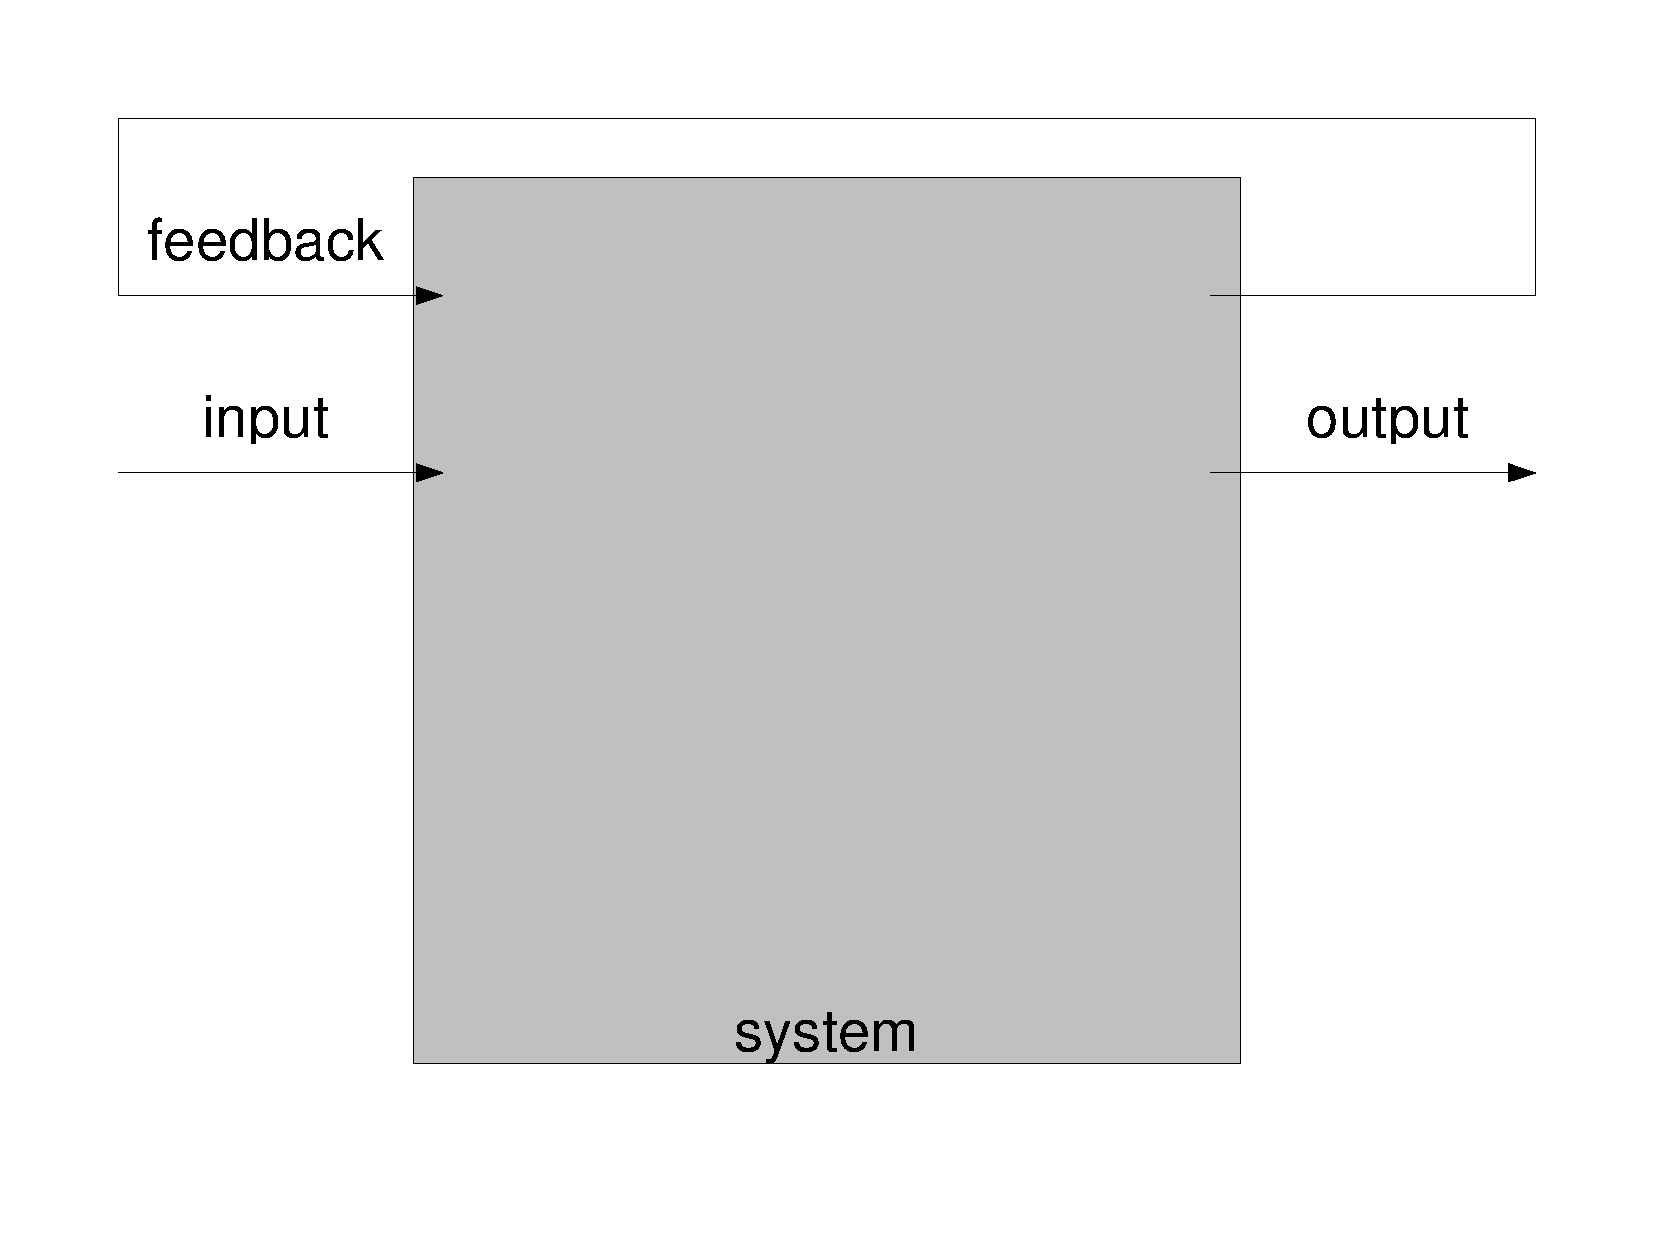
\includegraphics[scale=0.3,angle=-90]{graphic/blackbox.pdf}
        \caption{Closed Loop System with Feedback, modelled as Black Box}
        \label{blackbox_figure}
    \end{center}
\end{figure}

\newpage

A device controlling the behaviour of a system is called a \emph{Controller}.
Automation engineering uses electronic components such as \emph{Capacitor} and
\emph{Coil} to build controllers providing \emph{linear} (proportional),
\emph{differential} or \emph{integral} behaviour. In software engineering,
things are simpler. A computer program containing special mathematical
equations can simulate and control a system.

A software system's internal signal processing loop reads signals one by one,
from a signal memory (section \ref{knowledge_management_system_heading}).
While processing them, new signals may get created and placed in the signal
memory. This is how output results may be fed back to become a new input to the
software system.

%%
% $RCSfile: combinatoric_and_sequential_circuit.tex,v $
%
% Copyright (C) 2002-2008. Christian Heller.
%
% Permission is granted to copy, distribute and/or modify this document
% under the terms of the GNU Free Documentation License, Version 1.1 or
% any later version published by the Free Software Foundation; with no
% Invariant Sections, with no Front-Cover Texts and with no Back-Cover
% Texts. A copy of the license is included in the section entitled
% "GNU Free Documentation License".
%
% http://www.cybop.net
% - Cybernetics Oriented Programming -
%
% http://www.resmedicinae.org
% - Information in Medicine -
%
% Version: $Revision: 1.1 $ $Date: 2008-08-19 20:41:05 $ $Author: christian $
% Authors: Christian Heller <christian.heller@tuxtax.de>
%

\subsubsection{Combinatoric- and Sequential Circuit}
\label{combinatoric_and_sequential_circuit_heading}

\cite{wuttke}
Combinatoric Circuit (Stearing, Open Loop)
Sequential Circuit (Control, Closed Loop, Automat)
- internal state (output) is fed back to input
- necessary for conditions (if) in CYBOL
- a flag is set to true or false, as result of a comparison
- this flag is used as additional input to an operation which
only gets executed if the flag is true
- an input model for a CYBOL operation can represent an output model, at the same time;
similarly can an output represent an input (feedback loop);
the reference (path) to a knowledge model just has to be given as parameter of the operation;
it is up to the operation whether to use the referenced static model as input or output

%
% $RCSfile: input_output_and_rules.tex,v $
%
% Copyright (C) 2002-2008. Christian Heller.
%
% Permission is granted to copy, distribute and/or modify this document
% under the terms of the GNU Free Documentation License, Version 1.1 or
% any later version published by the Free Software Foundation; with no
% Invariant Sections, with no Front-Cover Texts and with no Back-Cover
% Texts. A copy of the license is included in the section entitled
% "GNU Free Documentation License".
%
% http://www.cybop.net
% - Cybernetics Oriented Programming -
%
% http://www.resmedicinae.org
% - Information in Medicine -
%
% Version: $Revision: 1.1 $ $Date: 2008-08-19 20:41:07 $ $Author: christian $
% Authors: Christian Heller <christian.heller@tuxtax.de>
%

\subsubsection{Input/Output and Rules}
\label{input_output_and_rules_heading}
\index{Data Structure}
\index{Enterprise Resource Planning System}
\index{ERP}
\index{Knowledge Model}
\index{Steady State}
\index{Converter containing Rules}
\index{Black Box}
\index{Logic Model}
\index{State Model}
\index{Information Flow}

In order to process data correctly, a system needs to know about their
\emph{Structure}. Software systems work with data belonging to some knowledge
model. Chapter \ref{knowledge_schema_heading} demonstrated how knowledge can be
modelled. Many applications keep their knowledge in special data files. Others,
such as \emph{Enterprise Resource Planning} (ERP) systems, retrieve their data
from a database. Even systems claiming to do nothing than pure data processing,
possibly using one operation only, rely on simple knowledge models, for at
least their \emph{Input/Output} (i/o) data.

Living systems rely on constantly exchanging information, energy, nutrients and
excretion products with their environment; they are never in a stationary, but
always in a \emph{Steady State}. A biological cell, for example, has inputs and
outputs and reacts in a certain manner which, after \cite{sengbusch}, is best
modelled with a \emph{Converter} containing \emph{Rules}, and treated as black
box. The cell's characteristic behaviour results from the way it relates inputs
to outputs.

\begin{figure}[ht]
    \begin{center}
        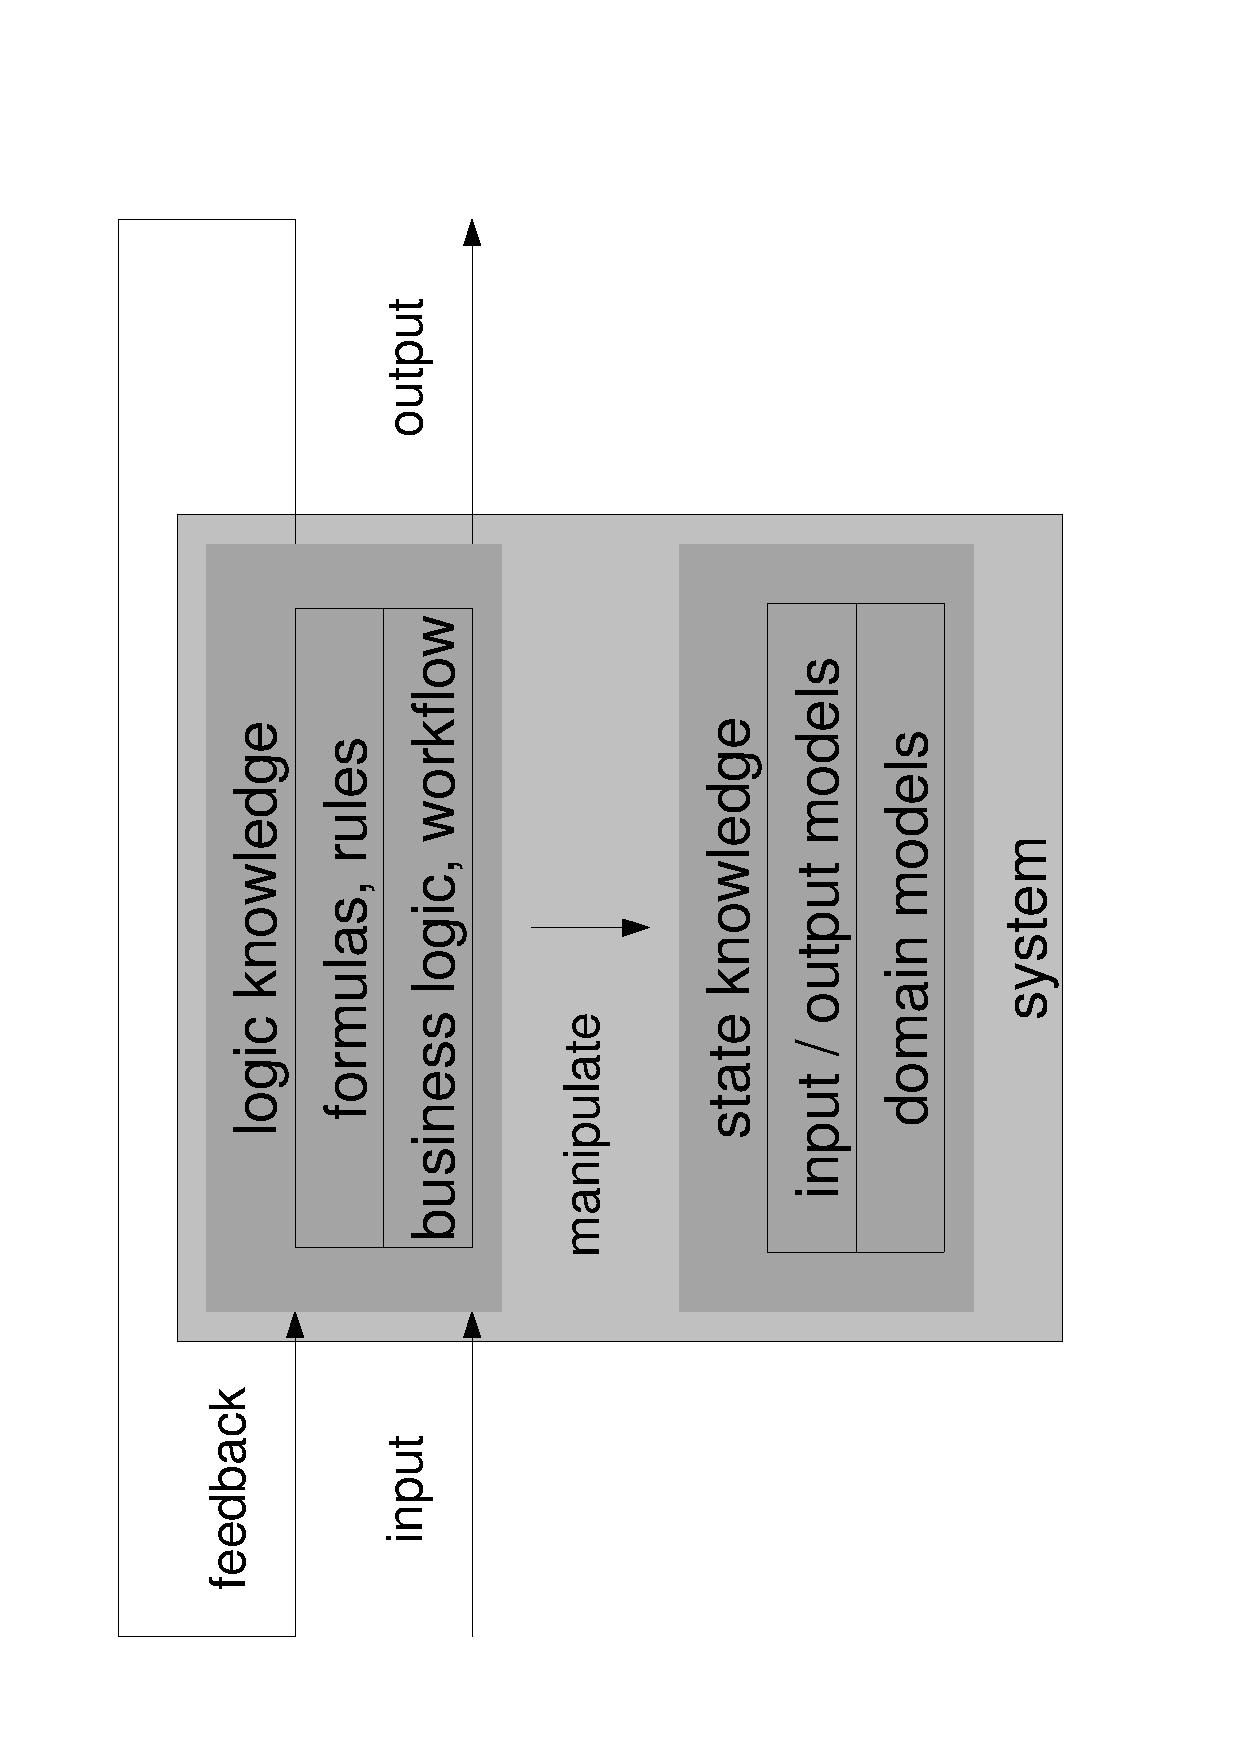
\includegraphics[scale=0.3,angle=-90]{graphic/manipulation.pdf}
        \caption{Logic translates between Input-, Domain- and Output States}
        \label{manipulation_figure}
    \end{center}
\end{figure}

Whilst figure \ref{blackbox_figure} illustrated the i/o flow of a system from
an \emph{outside} view, figure \ref{manipulation_figure} also considers the
state- and logic knowledge situated \emph{inside} a system. The arrow
indicating the information flow is directed from \emph{Logic-} towards
\emph{State} models, because the former manipulate the latter.

